%
% General structure for the revdetua class:
%
\documentclass[...]{revdetua}
\usepackage{graphicx}
\usepackage{float}

% listings to highlight code
\usepackage{pythonhighlight}

%
% Valid options are:
%
%   longpaper --------- \part and \tableofcontents defined
%   shortpaper -------- \part and \tableofcontents not defined (default)
%
%   english ----------- main language is English (default)
%   portugues --------- main language is Portuguese
%
%   draft ------------- draft version
%   final ------------- final version (default)
%
%   times ------------- use times (postscript) fonts for text
%
%   mirror ------------ prints a mirror image of the paper (with dvips)
%
%   visiblelabels ----- \SL, \SN, \SP, \EL, \EN, etc. defined
%   invisiblelabels --- \SL, \SN, \SP, \EL, \EN, etc. not defined (default)
%
% Note: the final version should use the times fonts
% Note: the really final version should also use the mirror option
%

\begin{document}

\Header{1}{25}{janeiro}{2023}{0}
% Note: the month must be in Portuguese

\title{Most Frequent Letters}
\author{Eduardo Santos, nºmec 93107, eduardosantoshf@ua.pt} % or \author{... \and ...}
\maketitle

\begin{abstract}
The objective of this assignment was to identify the most frequent letters in text files  using different methods and to evaluate the quality of estimates regarding the exact counts. Three types of counters were implemented: an Exact Counter, a Decreasing Probability Counter, and a Frequent Counter. 
\end{abstract}

\begin{keywords}{Counting Exact Counter, Decreasing Probability Counter, Frequent Counter}
\end{keywords}

\section{Introduction}

\subsection{Decreasing Probability Counter}

The aim of a probabilistic counter is to count very large numbers using only a little space to store the counter. Counting a very large number of events using an exact counter will result in a large memory usage, which is something that should be avoided, as memory is expensive, and makes a program less efficient. To mitigate this problem, probabilistic counters were created. So, for each call to an increment method on the counter, its actual value is updated with probability \textit{p}. Using this method, we are trading accuracy for the ability to count up to very large numbers with little storage space.

Even though nowadays memory is no longer scarce, this approach is still useful when treating/counting massive data volumes, when there is a need for quick and memory-efficient processing.

\subsection{Frequent Counter}

A streaming algorithm is an algorithm for processing data streams in which the input is presented as a sequence of items and can be examined in only a few passes, typically just one.
The frequent problem happens when, given a sequence of items, we want to identify those which occur most frequently. This can also be expressed as finding all items whose frequency exceeds a specified fraction of the total number of items.

\section{Problem Description}

The  goal of this assignment was to identify the most frequent letters in text files using different methods and to evaluate the quality of estimates regarding the exact counts.

In order to accomplish that, three different approaches were developed and tested:
\begin{itemize}
    \item exact counter
    \item approximate counter - decreasing probability counter with probability \(\frac{1}{\sqrt{2}^k}\)
    \item frequent counter - Misra \& Gries algorithm to identify frequent items in data streams
\end{itemize} 

The testing involved an analysis of the computational efficiency and limitations of the developed approaches was carried out, in terms of absolute and relative errors, computing the mean, minimum, and maximum of each error, as well as computing the standard deviation and variance.
Finally, for each method, the most frequent letters were identified, checking if they were in the same relative order.

\section{Implementation Description}

Running the \textbf{main.py}, with the \textbf{--help} flag, a few running options are presented.

\begin{figure}[!htb]
    \centering
    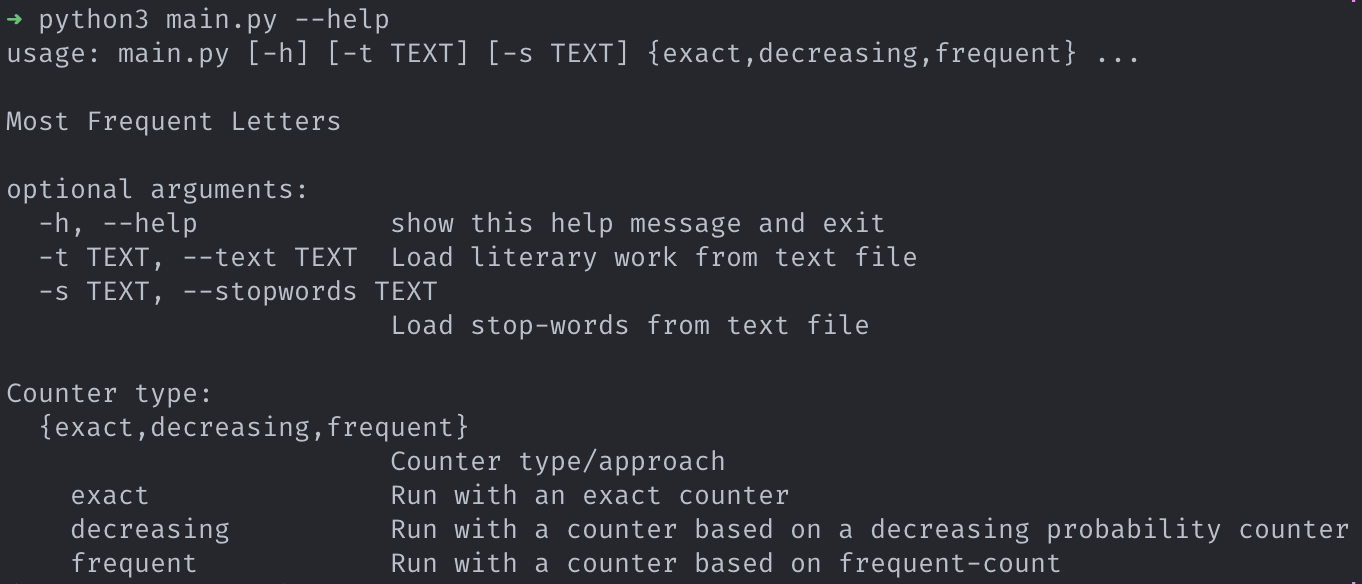
\includegraphics[width=1\columnwidth]{./figures/usage}
    \caption{Help Menu of the Main Program}
    \label{fig: Help Menu}
\end{figure}

The \textbf{-t} flag represents the filename of the literary work to be read and processed by the program, which can be found inside the \textbf{/texts/} directory. The \textbf{-s} flag represents the filename of the stopwords to be ignored when processing the text file. The stopwords files can be found inside the \textbf{/stopwords/} directory. After the previous parameters, we have to specify the counter type to be computed, using one of the following:
\begin{itemize}
    \item \textbf{exact} - count using the exact counter
    \item \textbf{decreasing} - count using the decreasing probability counter (with probability \(\frac{1}{\sqrt{2}^k}\))
    \item \textbf{frequent} - count using the frequent counter (we must also specify the \textit{k} parameter, using the flag \textbf{-k})
\end{itemize}

The \textbf{counter.py} contains the main logic of the solution, using the \textbf{ABC}\cite{abstract_base_classes} (Abstract Base Classes) Python module, the \textbf{ExactCounter}, \textbf{DecreasingProbabilityCounter}, and \textbf{FrequentCounter} classes extend the \textbf{Counter} parent class, using an OOP (object-oriented programming) model.
The \textbf{Counter} class contains the following methods:
\begin{itemize}
    \item \textit{read\_letters(self)}
\end{itemize}

\begin{python}
def read_letters(self):
        with open(self.filename, 'r') as file:
            while True:
                line = file.readline()

                # ignore the Project Gutenberg's file headers
                if line.strip() in [header.value for header in Headers]: break
                
            while line:
                line = file.readline()

                # ignore the Project Gutenberg's file footers
                if line.strip() in [footer.value for footer in Footers]: break

                for words in line.split():
                    # remove all stop-words and punctuation marks
                    for word in regex.findall('\p{alpha}+', words):
                        for letter in word:
                            self.parsed_letters.append(letter.upper())
\end{python}


Inside the 

\section{Results and Discussion}


\section{Conclusion}


\begin{thebibliography}{9}


% https://en.wikipedia.org/wiki/Approximate_counting_algorithm
% https://www.algorithm-archive.org/contents/approximate_counting/approximate_counting.html
% https://people.csail.mit.edu/rrw/6.045-2020/encalgs-mg.pdf
% https://medium.com/nerd-for-tech/the-streaming-model-and-how-to-estimate-the-most-frequent-elements-with-the-misra-gries-algorithm-c880bbe7218b
% https://en.wikipedia.org/wiki/Streaming_algorithm#:~:text=In%20computer%20science%2C%20streaming%20algorithms,passes%20(typically%20just%20one).
% https://github.com/jesuszarate/FrequentItems/blob/master/MisraGries/misra-gries.py
% https://github.com/joshuaeitan/misra_gries/blob/master/misra_gries/misra_gries.py
% 

\bibitem{regular_expressions}
Python Software Foundation. (Dec 22, 2022). re — Regular expression operations. \url{https://docs.python.org/3/library/re.html}

\bibitem{abstract_base_classes}
Python Software Foundation. (Dec 22, 2022). abc — Abstract Base Classes. \url{https://docs.python.org/3/library/abc.html}

\end{thebibliography}


% use a field named url or \url{} for URLs
% Note: the \bibliographystyle is set automatically

\end{document}
